\documentclass[aps,prd,onecolumn,nofootinbib,floatfix]{revtex4-2}
\usepackage{amsmath,amssymb}
\usepackage{graphicx}
\usepackage{booktabs}
\usepackage[hidelinks]{hyperref}
\graphicspath{{figures/}}
\newcommand{\degr}{^\circ}
\renewcommand{\thetable}{S\arabic{table}}
\renewcommand{\thefigure}{S\arabic{figure}}
\renewcommand{\thesection}{S\arabic{section}}

\begin{document}

\title{Supplemental Material for ``Unbiased Hubble-constant inference from strongly lensed gravitational waves with identified host galaxies''}
\maketitle

This Supplemental Material lists the true values and the posteriors of every analyzed system (Sec.~\ref{sec:all}) and shows the posteriors of all parameters of one O5 system (Sec.~\ref{sec:o5}), which complements the ET system of Appendix~A of the paper. The file \texttt{persystem.csv} gives, for every system, the true values and the 5\%, 50\% and 95\% posterior quantiles of all parameters of the joint parameter estimation of the GW data and of the GW+EM analysis; its columns are described in Sec.~\ref{sec:csv}. Section, equation and figure numbers without the prefix S refer to the paper.

\section{Every analyzed system}
\label{sec:all}
Table~S3, on the last pages of this document, lists for each of the 60 ET and 59 O5 systems, the true lens and source parameters, the results of the joint parameter estimation of the two GW images that enter the GW likelihood of the $H_0$ analysis (Sec.~IV\,A), and and the results of the GW+EM analysis with the lens model of the simulated family, normalized source prior and selection term, as in Fig.~5. The labels $A$ and $B$ of the two GW images are those of the GW data.

Table~\ref{tab:coverage} summarizes the calibration over the systems: the fraction of systems whose 90\% interval contains the true value. For calibrated posteriors this fraction is 0.90, and it lies within $\pm0.06$ of 0.90 in 90\% of samples of 60 systems. Most parameters are within this range. For ET, the apparent distance of image $A$ (0.83) and its arrival time (0.78) are covered less often; the arrival time is not used by the $H_0$ analysis, and removing the apparent distance from the GW likelihood changes the per-system $h$ by a median of only 0.16 standard deviations (Sec.~V\,D). For O5, the mass ratio (0.78) and the inclination (0.81) are covered less often, while the magnification ratio, the apparent distance and the delay, which enter the $H_0$ analysis, are covered for 0.88--0.93 of the systems. The coverage of $h$ for O5, 0.83, is the shortfall of strongly magnified systems discussed in Sec.~V\,B and Appendix~B.

\begin{table}[h]
\caption{Fraction of systems whose 90\% interval contains the true value. GW parameters: joint parameter estimation (ET with the sky position of the host, O5 with a free sky position); for the arrival time, 51 O5 systems (the others did not store it). GW+EM: model of the simulated family, with the selection term for $h$.\\ $^a$ Median $\pm1.645$ standard deviations, for the 15 (ET) and 14 (O5) EPL+shear systems.}
\label{tab:coverage}
\begin{tabular}{@{}lcc@{}}
\toprule
Parameter & ET (60) & O5 (59)\\
\midrule
Chirp mass $\mathcal M$ & 0.95 & 0.90\\
Mass ratio $m_2/m_1$ & 0.78 & 0.78\\
Spin $\chi_1$ & 0.93 & 0.92\\
Spin $\chi_2$ & 0.97 & 1.00\\
Inclination $\theta_{JN}$ & 0.90 & 0.81\\
Apparent distance $D_A$ & 0.83 & 0.88\\
$\ln|\mu_B/\mu_A|$ & 0.87 & 0.92\\
Arrival time $t_A$ & 0.78 & 0.92\\
Delay $\Delta t$ & 0.92 & 0.93\\
$\mu_A$ (GW+EM) & 0.92 & 0.88\\
$h$ (GW+EM) & 0.92 & 0.83\\
Slope $\gamma'$ (GW+EM, EPL+shear)$^a$ & 0.93 & 0.86\\
\bottomrule
\end{tabular}

\end{table}

\section{Posteriors of all parameters of an O5 system}
\label{sec:o5}
Figures~\ref{fig:cornergw} and \ref{fig:cornerlens} and Table~\ref{tab:fullpost} show the posteriors of all parameters of a typical O5 system, as Appendix~A of the paper does for an ET system. The lens, an EPL+shear galaxy at $z_l=0.82$ with $\theta_E=0.60$\,arcsec, $q=0.71$ and $\gamma'=1.88$, produces four images of a source at $z_s=1.44$. The two detected GW images are the merging pair near a fold caustic: image $A$ at a saddle point with $\mu_A=-10.9$, image $B$ at a minimum with $\mu_B=13.0$, a delay of 5.6 hours and network SNRs of 28 and 24.

With a free sky position, the joint parameter estimation places the source within $4.5\degr$ of its true position (90\% probability). The source is massive and unequal (detector-frame chirp mass $102\,M_\odot$, mass ratio 0.32), so that the higher harmonics are strong and the Morse indices are resolved: $(n_A,n_B)=(\frac12,0)$ has probability 0.99, compared with 0.53 for the ET system of Appendix~A. Three of the 13 continuous parameters lie just outside their 90\% intervals: the right ascension, the apparent distance of image $A$ (true value 3.22\,Gpc, interval 3.26--4.09\,Gpc) and the delay. The delay, which is defined at the geocenter, is offset by $-0.9$\,ms and is correlated with the right ascension (correlation coefficient $-0.6$); at the true sky position the expected offset is $-0.4$\,ms. Either is a fraction $4\times10^{-8}$ of the delay.

The four images fix the Einstein radius to 1\% and, through the isothermal relation, the velocity dispersion to 1\%. The slope, $2.01$ against the true $1.88$, is constrained little more than by its prior, and $h$ follows it (correlation coefficient 0.69 between $\gamma'$ and $\ln h$). The magnifications are measured to 25\% (standard deviation of $\ln|\mu|$). As for the ET system, the posterior of $\kappa_{\rm ext}$ equals its prior, and the lens center is determined mainly by the light center; the true center lies 1.8 prior standard deviations from it, and both of its coordinates lie just outside their 90\% intervals. Without the selection term $h=1.01$ (90\% interval 0.80--1.26); with it, $h=0.96$ (0.76--1.20). For O5, where the selection fraction varies as $\alpha\propto h^{2.7}$ (Sec.~IV\,D), the selection term matters even for a single system, whereas for the ET system it changes $h$ by only 0.01.

\begin{table}[h]
\caption{True values, medians and 90\% intervals of all parameters of the O5 system (EPL+shear 0025278). Angles are in radians; $t_A$ is the geocentric arrival time of image $A$ and $\Delta t$ the delay of image $B$. For the Morse indices, the posterior probabilities of the two combinations found are given; $h$ is given without the selection term.}
\label{tab:fullpost}
\begin{tabular*}{\linewidth}{@{\extracolsep{\fill}}lccc@{}}
\toprule
Parameter & Truth & Median & 90\% interval\\
\midrule
\multicolumn{4}{@{}l}{\emph{GW: joint parameter estimation, free sky position}}\\
Chirp mass $\mathcal M$ ($M_\odot$) & $101.647$ & $106.625$ & $[96.716,\ 113.504]$\\
Mass ratio $m_2/m_1$ & $0.32$ & $0.38$ & $[0.31,\ 0.43]$\\
Spin $\chi_1$ & $0.02$ & $-0.05$ & $[-0.21,\ 0.07]$\\
Spin $\chi_2$ & $-0.16$ & $-0.26$ & $[-0.71,\ 0.13]$\\
Inclination $\theta_{JN}$ & $2.02$ & $2.01$ & $[1.87,\ 2.19]$\\
Polarization $\psi$ & $0.85$ & $0.81$ & $[0.71,\ 0.95]$\\
Phase $\phi_c$ & $1.30$ & $1.10$ & $[0.83,\ 1.38]$\\
Right ascension $\alpha$ & $3.139$ & $3.181$ & $[3.152,\ 3.207]$\\
Declination $\delta$ & $0.385$ & $0.355$ & $[0.314,\ 0.393]$\\
$D_A=d_L/\sqrt{|\mu_A|}$ (Gpc) & $3.22$ & $3.65$ & $[3.26,\ 4.09]$\\
$\ln|\mu_B/\mu_A|$ & $0.18$ & $0.57$ & $[0.14,\ 1.08]$\\
$\delta t_A=t_A-t_A^{\rm true}$ (ms) & $0.000$ & $-1.830$ & $[-4.330,\ 0.739]$\\
$\delta\Delta t=\Delta t-\Delta t^{\rm true}$ (ms) & $0.000$ & $-0.885$ & $[-1.478,\ -0.343]$\\
Morse indices $(n_A,n_B)$ & $(\tfrac12,0)$ & \multicolumn{2}{c}{$(\tfrac12,0)$: 0.99; $(1,\tfrac12)$: 0.01}\\
\midrule
\multicolumn{4}{@{}l}{\emph{GW+EM: EPL+shear lens model, $\kappa_{\rm ext}$ and $h$}}\\
$\theta_E$ (arcsec) & $0.595$ & $0.597$ & $[0.586,\ 0.608]$\\
Radial slope $\gamma'$ & $1.88$ & $2.01$ & $[1.85,\ 2.23]$\\
Axis ratio $q$ & $0.71$ & $0.71$ & $[0.63,\ 0.78]$\\
Orientation $\varphi$ & $2.80$ & $2.84$ & $[2.70,\ 3.00]$\\
Shear $\gamma_{\rm ext}$ & $0.042$ & $0.044$ & $[0.018,\ 0.089]$\\
Shear orientation $\varphi_{\rm ext}$ & $1.30$ & $1.25$ & $[0.75,\ 1.71]$\\
Center $x_c$ (arcsec) & $-0.009$ & $-0.022$ & $[-0.033,\ -0.010]$\\
Center $y_c$ (arcsec) & $-0.035$ & $-0.008$ & $[-0.027,\ 0.011]$\\
$\sigma_v$ (km\,s$^{-1}$) & $251$ & $251$ & $[249,\ 254]$\\
$\kappa_{\rm ext}$ & $0.000$ & $0.000$ & $[-0.042,\ 0.037]$\\
$\mu_A$ & $10.90$ & $9.72$ & $[6.52,\ 14.39]$\\
$|\mu_B|$ & $13.02$ & $12.10$ & $[8.26,\ 17.60]$\\
$h=H_0/H_0^{\rm true}$ & $1.00$ & $1.01$ & $[0.80,\ 1.26]$\\
\bottomrule
\end{tabular*}

\end{table}

\begin{figure*}
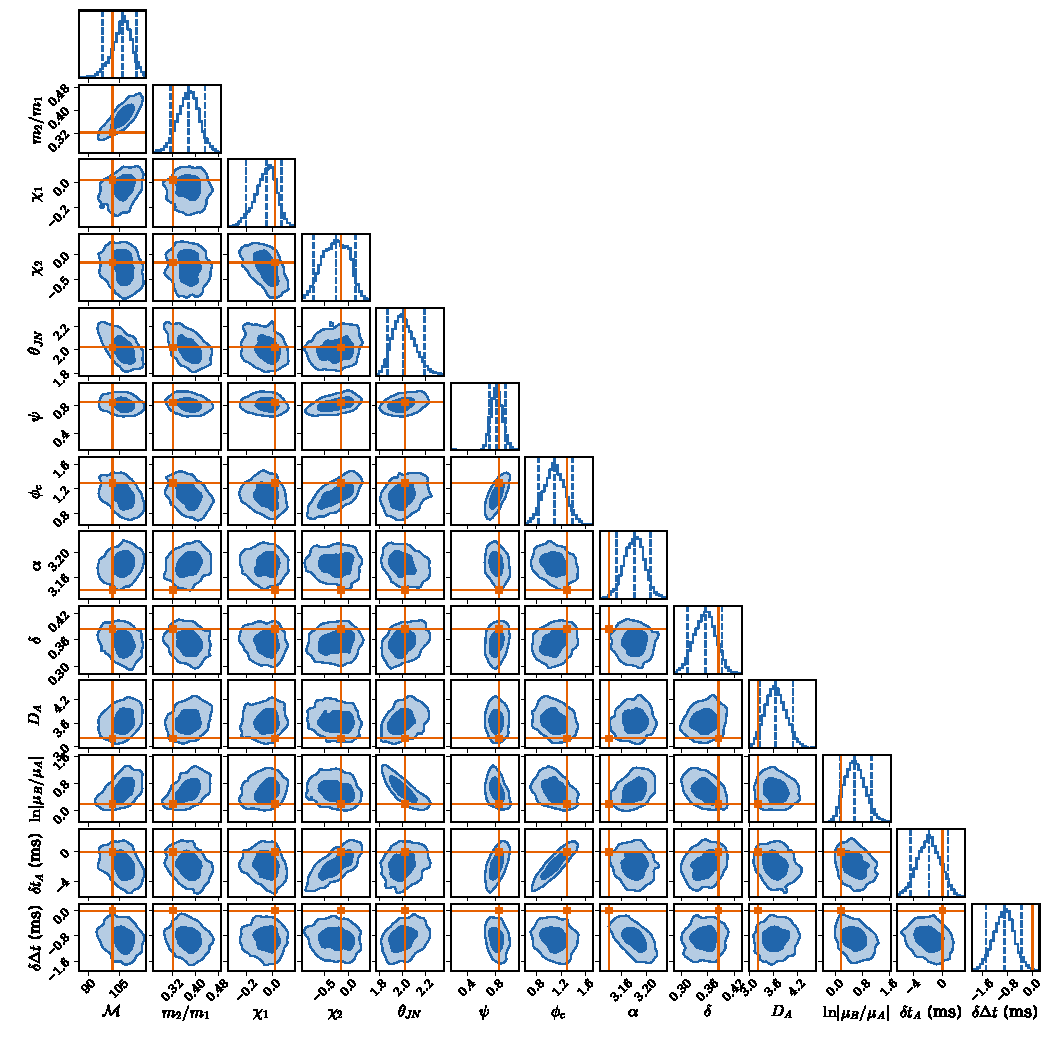
\includegraphics[width=\textwidth]{fig_corner_gw_O5.pdf}
\caption{Joint parameter estimation of the two GW images of the O5 system, with a free sky position: detector-frame chirp mass $\mathcal M$ (in $M_\odot$), mass ratio, aligned spins, inclination, polarization angle and phase, right ascension and declination (in rad), apparent distance of image $A$ (in Gpc), magnification ratio, and the offsets of the arrival time of $A$ and of the delay from their true values (in ms). Contours enclose 50\% and 90\% of the posterior; dashed lines mark the medians and 90\% intervals, and orange lines the true values.}
\label{fig:cornergw}
\end{figure*}

\begin{figure*}
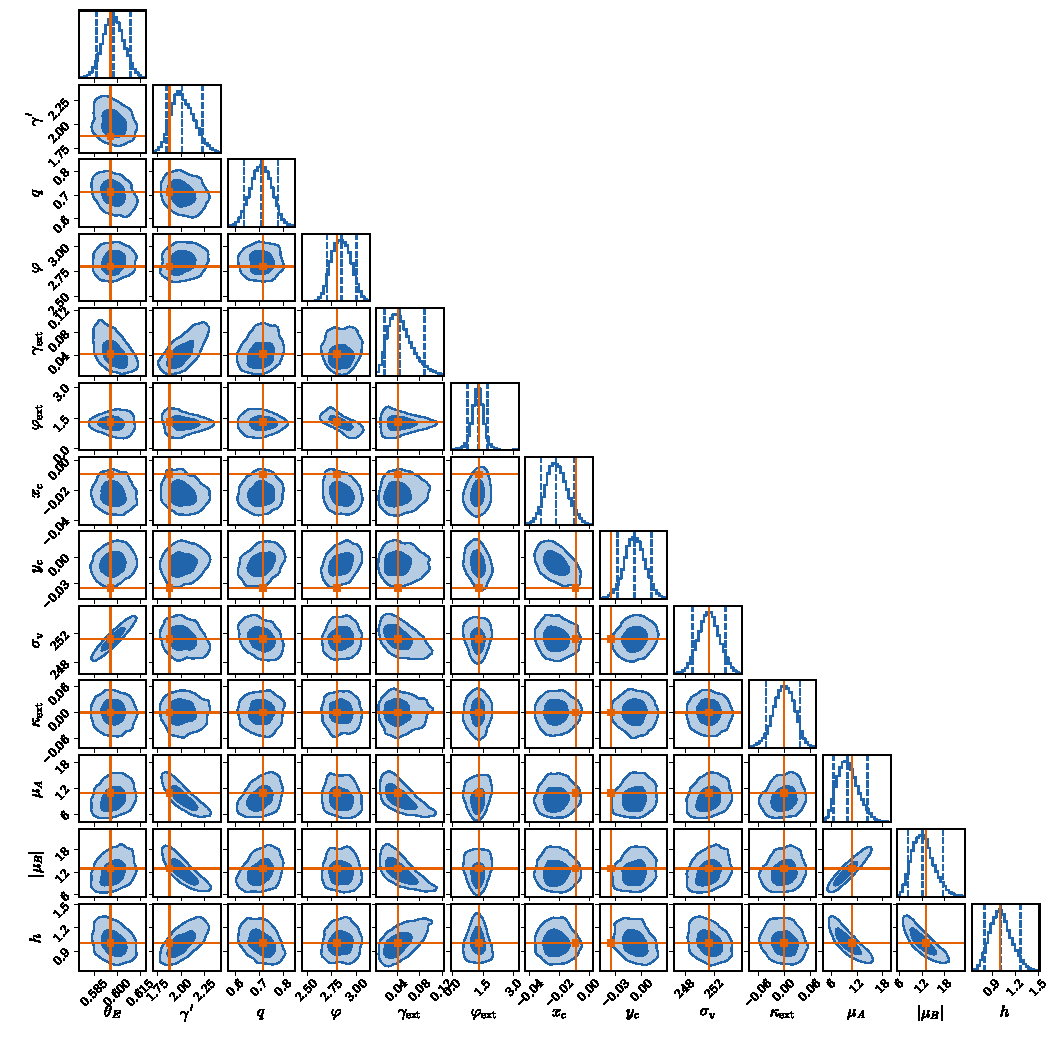
\includegraphics[width=\textwidth]{fig_corner_lens_O5.pdf}
\caption{GW+EM posterior of the O5 system with the EPL+shear model: Einstein radius and lens center (in arcsec), slope, axis ratio and orientation of the mass, shear strength and orientation, velocity dispersion (in km\,s$^{-1}$), external convergence, the magnifications of the two images, and $h$ (without the selection term). Lines and contours as in Fig.~\ref{fig:cornergw}.}
\label{fig:cornerlens}
\end{figure*}

\section{The file \texttt{persystem.csv}}
\label{sec:csv}
One row per system. Identification: \texttt{scenario}, \texttt{family}, \texttt{event\_id}. True values: \texttt{z\_l}, \texttt{z\_s}, \texttt{theta\_E} (arcsec), \texttt{gamma\_true}, \texttt{q\_true}, \texttt{n\_images}, \texttt{sep\_arcsec} (separation of the two GW images), \texttt{dt\_days}, \texttt{d\_L\_Mpc}, source-frame masses \texttt{m1\_src}, \texttt{m2\_src}, optimal network SNRs \texttt{snr\_a}, \texttt{snr\_b}, Morse indices \texttt{morse\_a\_true}, \texttt{morse\_b\_true} and magnifications \texttt{mu\_a\_true}, \texttt{mu\_b\_true}. Joint parameter estimation, each with \texttt{\_true}, \texttt{\_q05}, \texttt{\_q50}, \texttt{\_q95}: \texttt{chirp\_mass} (detector frame, $M_\odot$), \texttt{mass\_ratio}, \texttt{chi\_1}, \texttt{chi\_2}, \texttt{theta\_jn}, \texttt{psi}, \texttt{phase}, \texttt{D\_A\_Mpc}, \texttt{ln\_mu\_rel} ($\ln|\mu_B/\mu_A|$), \texttt{dt\_offset\_ms} and \texttt{tA\_offset\_ms} (offsets of the delay and of the arrival time of $A$ from their true values); for O5 the median and 90th percentile of the sky offset, \texttt{sky\_offset\_deg\_q50}, \texttt{sky\_offset\_deg\_q90}; the posterior probabilities of the true Morse indices, \texttt{P\_morse\_true}, and of their true difference, \texttt{P\_dmorse\_true}. GW+EM analysis with the model of the simulated family: \texttt{mu\_a\_gwem\_q05/q50/q95}, \texttt{h\_q05/q50/q95} (with the selection term), \texttt{h\_nosel\_q05/q50/q95} (without), and for EPL+shear lenses the slope \texttt{gamma\_gwem\_median}, \texttt{gamma\_gwem\_sd}. Eight O5 parameter-estimation runs did not store the phase and the arrival time; these entries are empty.

\end{document}
